\subsection{16-bit Kogge-Stone Adder}
The Kogge-Stone adder consists of several simple blocks connected in a complex way, as can be seen in appendix \ref{app:ks_block}. The adder has been significantly changed since the high-level design phase. The \textit{yellow} block has been split into two blocks \textit{yellow\_inv\_in} and \textit{yellow\_inv\_out}, which can be seen in \ref{fig:yellow_opt}. The \textit{yellow\_inv\_in} block takes inverted input signals and gives non-inverting output. The \textit{yellow\_inv\_out} block takes non-inverted intputs and gives inverting output. This arrengement saves a lot of gates. The \textit{yellow\_carry} block has been split in the same way. 

Because of the inverting signals from \textit{yellow\_inv\_out} some \textit{sum} blocks have been replaced with XNOR gates. A couple of inverters have also been added in some places.

All transistors in the adder are minimum sized since the gates have a low fan out.

\begin{figure}[H]
  \centering
  \captionsetup{justification=centering}
  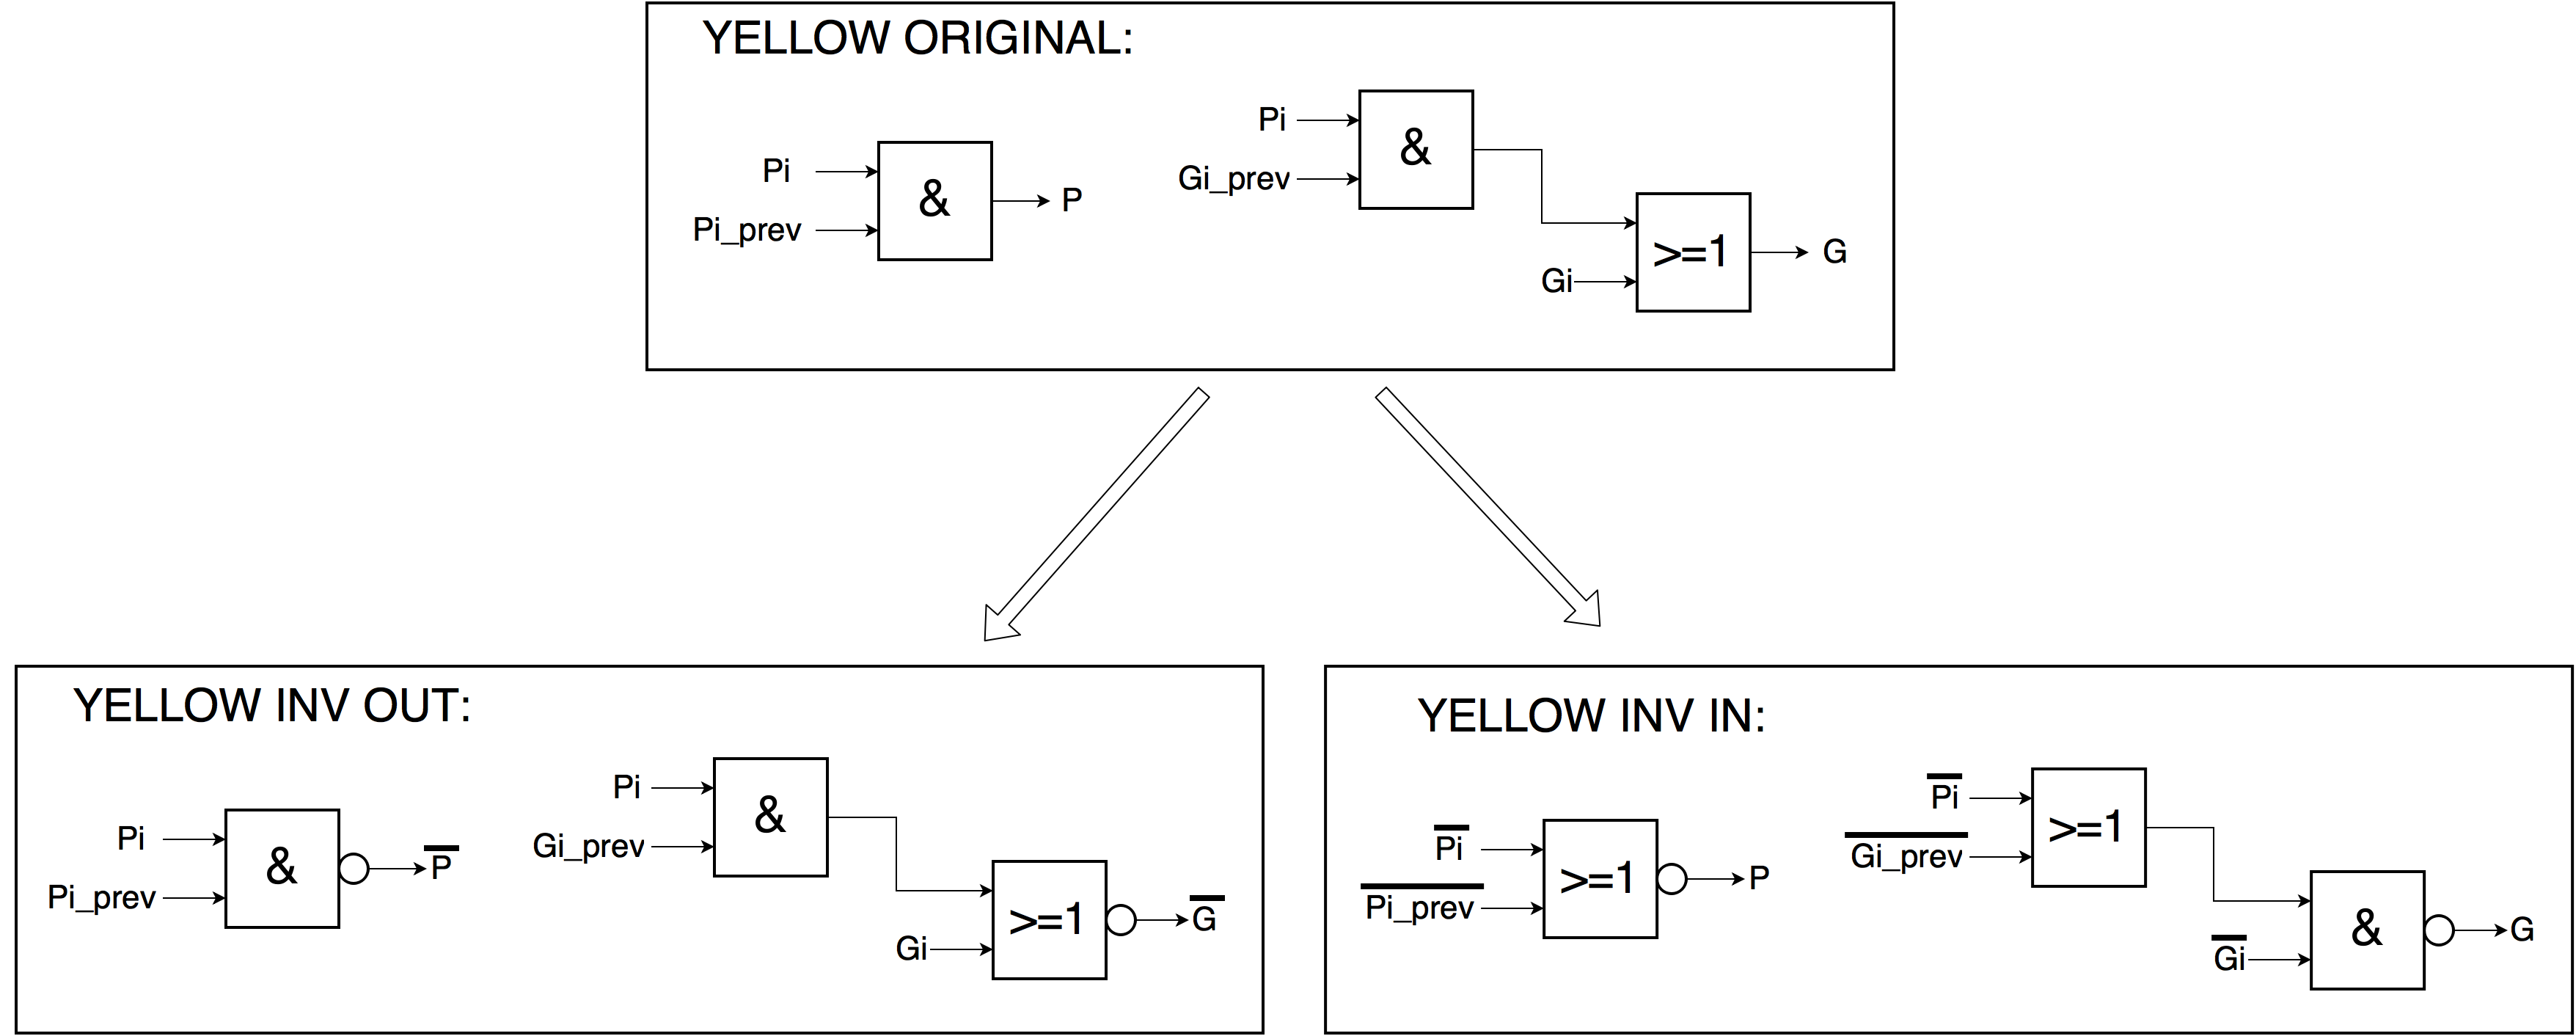
\includegraphics[scale=0.2]{../figures/yellow_opt}
  \caption{The new yellow blocks.} \label{fig:yellow_opt}
\end{figure}

\todo{Bild på generate gates osv}

\subsection{Comparator}
The comparator consists of 17 2-input XNOR gates where one bit of each number is fed into each gate. The output from the XNOR gates are fed into a couple of AND gates which generates the final output. The comparator is 17 bits wide since it compares two 16 bit numbers plus their carry bits. The logic table of the XNOR gates is shown in table \ref{tab:xnor}.

\begin{table}[H]
  \caption{Logic table of XNOR block.}
  \centering
  \begin{tabular}{cc|c}
    \toprule
    $A_i$ & $B_i$ & $Y = \overline{(A_i \oplus B_i)}$ \\
    \midrule
    0 & 0 & 1 \\
    0 & 1 & 0 \\
    1 & 0 & 0 \\
    1 & 1 & 1 \\
    \bottomrule
    \label{tab:xnor}
  \end{tabular}
\end{table}
